%%%%%%%%%%%%%%%%%%%%%%%% CAB432 Group Report %%%%%%%%%%%%%%%%%%%%%%%

%BEGIN_FOLD
% Disclaimer: You HAVE to use this. This is a not simple starting point, all libraries and titles were recreated for fit group Assignment, same way it was in EGB342. If something does not work... Well, you all know who to blame.

% This sets the style of the document, you can use different built in styles, create your own .cls files or download ones from the Internet. This one is fairly standard to use
\documentclass[12pt]{article}
\usepackage[natbibapa]{apacite}


%%%%%%%%%%%%%%%%%%%%%%%%%%%%% Packages %%%%%%%%%%%%%%%%%%%%%%%%%%%%%%

% This package is handy for captioning figures, you can set caption style here as well
\usepackage[font={small,it}]{caption}
\usepackage[a4paper, portrait, margin=0.8in,top=2cm,bottom=2cm,]{geometry}
\usepackage{bigstrut}

% This is important for position images as latex will put your image where it best fits unless you tell it otherwise
\usepackage{float}
\usepackage{wrapfig}

% If you want images this is necessary
\usepackage{graphicx}
\usepackage{subcaption}
\graphicspath{{./images}}
\usepackage{hyperref}
\usepackage{color}
\usepackage{xcolor}
\hypersetup{colorlinks=true}
\hypersetup{linkcolor=blue}
\newcommand\PlaceText[3]{%
\begin{tikzpicture}[remember picture,overlay]
\node[outer sep=0pt,inner sep=0pt,anchor=south west] 
  at ([xshift=#1,yshift=-#2]current page.north west) {#3};
\end{tikzpicture}%
}
% You can use this to set your margin size
%\usepackage[margin=25mm]{geometry}

% Allows you to do things such as headers and footers
\usepackage{fancyhdr}

% This needs to be in here if you want to set up your document with more than one column in sections 
\usepackage{multicol}

% Here are a few packages that help with formatting equations, you may not need to use this but I find align* from amsmath particularly useful
\usepackage{amsmath,amssymb,amsthm,textcomp,amsfonts,amsthm,mathrsfs}
\usepackage{xparse}% http://ctan.org/pkg/xparse
\NewDocumentCommand{\ceil}{s O{} m}{%
  \IfBooleanTF{#1} % starred
    {\left\lceil#3\right\rceil} % \ceil*[..]{..}
    {#2\lceil#3#2\rceil} % \ceil[..]{..}
}

% Enhances Latex`s cross referencing
\usepackage{cleveref}
\usepackage{hyperref}
\hypersetup{colorlinks=true}
\hypersetup{linkcolor=blue}
\usepackage{xcolor}
\usepackage{physics}
\usepackage{gensymb}
\usepackage{mathrsfs}

% Also not necessary but I find it handy when formatting arrays and matrices
\usepackage{array}
\usepackage{xfrac}
\usepackage{enumitem}

%% These packages you`ll need to download a .sty file before you can use

% This allows really nice formatting for MATLAB code.
\usepackage[numbered,framed]{mcode}
\usepackage{mathrsfs}
\usepackage{hyperref}
\hypersetup{colorlinks=true}
\hypersetup{linkcolor=blue}
\usepackage{xcolor}
\usepackage{physics}
\usepackage{gensymb}

%% Feel free to add any more packages you want!!!
\usepackage{indentfirst}
\usepackage{parskip} 
\setlength\parindent{0pt}
%\setlength{\parskip}{1cm plus4mm minus3mm}
\usepackage{csquotes}
\usepackage{mathtools}
\newcommand{\Lim}[1]{\raisebox{0.5ex}{\scalebox{0.8}{$\displaystyle \lim_{#1}\;$}}}
\usepackage{wrapfig}
\usepackage{tabularx} % in the preamble

%%%%%%%%%%%%%%%%%%%%%%%%% Setup the document %%%%%%%%%%%%%%%%%%%%%%%%

\lstset{basicstyle=\scriptsize\ttfamily,breaklines=true}
\renewcommand{\thesubsection}{\thesection.\arabic{subsection}.}

\renewcommand{\thesubsubsection}{\indent \roman{subsubsection}}

\numberwithin{equation}{section} % Number equations within sections (i.e. 1.1, 1.2, 2.1, 2.2 instead of 1, 2, 3, 4)
\numberwithin{figure}{section} % Number figures within sections (i.e. 1.1, 1.2, 2.1, 2.2 instead of 1, 2, 3, 4)
\numberwithin{table}{section} % Number tables within sections (i.e. 1.1, 1.2, 2.1, 2.2 instead of 1, 2, 3, 4)

\newcommand{\horrule}[1]{\rule{\linewidth}{#1}} % Create horizontal rule command with 1 argument of height

\title{	
	\normalfont \normalsize 
	\textsc{Queensland University of Technology} \\ [25pt] 
	\horrule{0.5pt} \\[0.4cm] % Thin top horizontal rule
	\huge CAB432 - Assignment 1 \\ Mashup Project \\ % The assignment title
	\author{ Marat (Matt) Sadykov \small n9312706 \\ \\ Tutor: Jacob Marks \small \underline{marksj@qut.edu.au}}
	\date{\normalsize\today} % Today`s date or a custom date
	\horrule{2pt} \\[0.5cm] % Thick bottom horizontal rule
}

% Headers and footers
\pagestyle{fancy}
\fancyhf{}
\rhead{Mashup Project Report}
\lhead{CAB432 Cloud Computing}
\cfoot{Marat (Matt) Sadykov}
\cfoot{Page \thepage}
\cfoot{n9312706}

%END_FOLD
%%%%%%%%%%%%%%%%%%%%% Begin the Actual Document %%%%%%%%%%%%%%%%%%%%%
\begin{document}
\maketitle
\newpage
\tableofcontents
\newpage
%===================================================%
%													%
%============ Section 1 Introduction ===============%
%												    %
%===================================================%
\section{Introduction}	
%	\begin{enumerate}
%		\item Overall mashup purpose and description (1-2 Paragraphs)
%		\item List of service and data APIs to be utilised. Short description of API (1 paragraph)
%	\end{enumerate} error made int

	The aim of this project to provide users with some comfortable environment to plan their journeys. This planner will use one of the following API\footnote{Names contain hyperlinks to resource. Feel free to click}: 
	
	\begin{itemize}
		\item \href{https://developers.google.com/maps/documentation/}{Google Maps}
		\item \href{https://hackathon.expedia.com/docs/public/api/Flights Overview/}{Expedian} with \href{https://api.flightstats.com/flex/flightstatus/rest/v2/json/route/status/}{Flightstats} combined for one purpose.
		\item \href{https://developers.webcams.travel/\#webcams/list}{Webcam}
	\end{itemize}	
	A user will be able to choose a destination, view closes and cheapest flight information and makes a decision based on a picture from realtime webcameras (Maybe it is not as pretty, but it will give right feeling regarding destination). First and the important part is an interactive map, provided by Maps services. It will allow a user to change view between satellite and geographic, zoom in to view details and help to extract geographic locations. Next is the webcam, which produces some images or short video streams on some of the sights of the area. And the Main part is quick information on the closest flight regarding price, time and journey. The first experiment version is presented in Figure~\ref{fig:map}.	

	\subsection{World Map}
		The foundation for weekend planer environment is continental Map. Gladly, there is a high chance of finding a right Map provider. Two global websites, whose work offers an API for use cases are Google Maps and Yandex. If first is the global giant, who existed in the worldwide market for a while, second has the most popularity in Russian. Both of them will serve the primary purpose very well: establish a right environment for integrating other API. Besides, both services provide an excellent API to extend the scope of the current project. \\
		
		As a result, the Google Map API was chosen with a way presented in Figure~\ref{fig:gmaps}. To describe location, a centre point of the map must be chosen with longitude and latitude. In addition, API provides a good drawing environment, which allows places some images on top of the map, draw markers or lines from one location, to another. As a scope of this unit, only Australia will be chosen as working environment.
		
		\begin{figure}[H]
			\centering        
			\includegraphics[width=0.7\textwidth]{images/google-map}
			\caption{Google Maps API at 54 54 longitude and latitude.}
			\label{fig:gmaps}
		\end{figure}
		
	\subsection{Flight Management}
		To gather information about the possible flight tickets, there is a possibility of some context particular problems. Since the beginning of the project, the request for API keys may take longer than expected. Such services like Expedia provides some flight information, which may be used to gather closest flight information about time, prices, airports. Obtaining this information may become a trickier process. For example, if there will be no alternatives discovered, the best solution in this situation will be parsing web page with flight information. However, this approach goes beyond the scope of the assignment, it may prove itself as a good, but not easy, alternative.\\
		
		As a result, plans were achieved using Flightstat API in combination with Expedia. In order to produce request which can be handled by flight API, there were need in creating request in particular form. In this situation, Expedia was able to provide certain returns based on name of the city, as an example, the code below represent two predefined messages for requests. In some situation, during development process, Expedia refused  to give response, that is why those predefined cities were created, to avoid error possibility and not interrupt user. Figure~\ref{fig:depar} provides an example of the flight from Main City\footnote{The one which user picked as starting point} to destination.
		
		\begin{lstlisting}
			function def_(name) {
			
				if (name == 'brisbane') {
					return {
						displayName: '<B>Brisbane</B>, Queensland, AU',
						fullName: 'Brisbane (and vicinity), Queensland, Australia',
						lastSearchName: 'Brisbane, Queensland, Australia',
						shortName: '<B>Brisbane</B>, Queensland, AU',
						coordinates: {lat: '-27.458819',  long: '153.103613'},
						airport: 'BNE'
					};
				}
				
				if (name == 'sydney') {
					return {
						displayName: '<B>Sydney</B>, New South Wales, AU',
						fullName: 'Sydney (and vicinity), New South Wales, Australia',
						lastSearchName: 'Sydney, New South Wales, Australia',
						shortName: '<B>Sydney</B>, New South Wales, AU',
						coordinates: {lat:  '-33.86757', long: '151.20844'},
						airport: 'SYD'
				};
				...
				...
			}
		\end{lstlisting}
		\begin{figure}[H]
			\centering        
			\includegraphics[width=0.7\textwidth]{images/departure}
			\caption{Departure flights from Brisbane to Perth.}
			\label{fig:depar}
		\end{figure}
	\subsection{Location Explorer}
		$  $ \\
		
		To gather information unusually and present in on top of maps webcam service will be used. Generally, it contains Library of open web cameras located around the world. Instead of gathering all possible sources, webcam includes all of them in one place. It will allow extracting at least images, which were made very recent to a user request. An example of how data can be collected is displayed in Figure~\ref{fig:webcam}. \\
		
		As a result of hard work with Webcams API, it was possible to integrate a real time video playtghrough, fresh within 5-15 minutes. In case if need, streams can be switched to Day, Month or Year in Timeleps. Video Players also includes information about provider, link for connection and script for embed, in addition to full screen view. Figure~\ref{fig:webCam-adel} refers to their view~\footnote{Nothing inspires more than eye dropping over someones life, or an entire city.}.
		\begin{figure}[H]
			\centering        
			\includegraphics[width=0.7\textwidth]{images/webcam-adel}
			\caption{Departure flights from Brisbane to Perth.}
			\label{fig:webCam-adel}
		\end{figure}
\newpage		
%===================================================%
%													%
%============ Section 2 Use Cases ==================%
%												    %
%===================================================%
\section{Use Cases}
	\subsection{Trip Planner}
		The main expected advantage of this service is to \textbf{plan trips to several places} on one Map, instead of planning on the official website, comparing each ticket one by one. This comparison gives user possibility select option flexibally choose places and time.
		
		\begin{figure}[H]
			\centering        
			\includegraphics[width=0.7\textwidth]{images/Google-web}
			\caption{Departure flights from Brisbane to Perth.}
			\label{fig:webCam}
		\end{figure}
		\begin{figure}[H]
			\begin{subfigure}[b]{0.52\textwidth}
				\centering
				\includegraphics[width=\linewidth]{images/flight-ad}
				\caption{Flights to Adelaide.}
				
			\end{subfigure}
			\begin{subfigure}[b]{0.52\textwidth}
				\centering
				\includegraphics[width=\linewidth]{images/flight-sd}
				\caption{Flights to Sydney.}
				
			\end{subfigure}
			\caption{Choosing most efficient flight.}
		\end{figure}
	\subsection{Exploring area with cameras}
		Web cameras spread around cities all other the place. Some of them may contain boring traffic exploration, another some beautiful views. Comparing to high-quality images on other services, webcam takes real-time shoots. The original intention is to allow the user to plan short weekend trips. \textbf{There is no better way to make decision rather take a small pick into a city of destination.}
		\begin{figure}[H]
			\centering        
			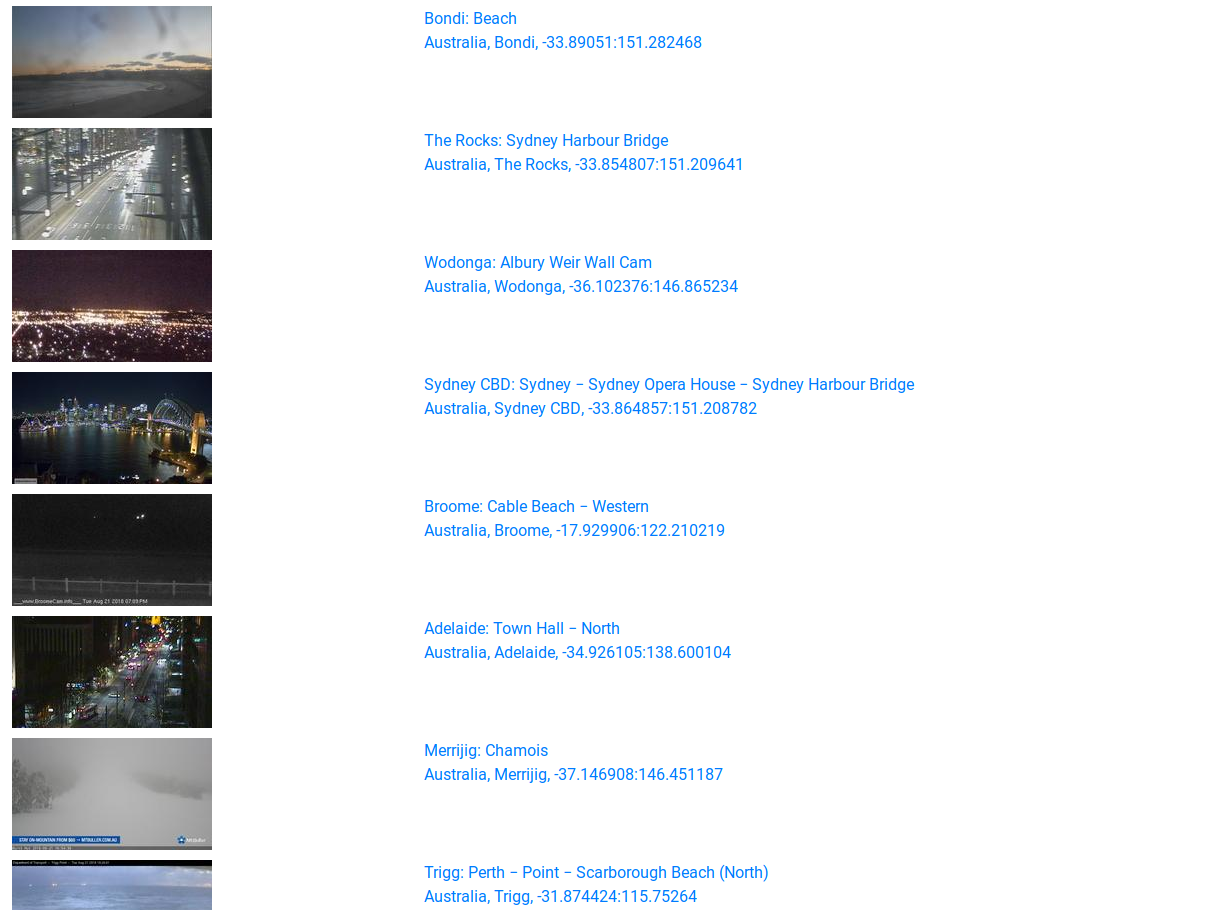
\includegraphics[width=0.7\textwidth]{images/webcam}
			\caption{First test print with API use.}
			\label{fig:webcam}
		\end{figure}
		By choosing one cities, he can visualise video of current situation in predefined area.
		\begin{figure}[H]
			\begin{subfigure}[b]{0.52\textwidth}
				\centering
				\includegraphics[width=\linewidth]{images/webcam-ch}
				\caption{Choose from server.}
				
			\end{subfigure}
			\begin{subfigure}[b]{0.52\textwidth}
				\centering
				\includegraphics[width=\linewidth]{images/webcam-lv}
				\caption{Watch live stream.}
				
			\end{subfigure}
			\caption{Webcam in Melbourne}
		\end{figure}
	
	\subsection{Exploring area with Google Maps}
		The usage of Google Maps allowed change map view to the most suitable for user, as well as tossing virtual itself into any area on the map.
		\begin{figure}[H]
			\centering        
			\includegraphics[width=0.7\textwidth]{images/map-toss}
			\caption{Pick location to explore with Google.}
			\label{fig:toss}
		\end{figure}
	\subsection{Weekend planner}
	In addition to flight management and camera exploration, some of \textbf{the Maps services} can be used to make decisions on sight. For example, explore the streets a destination in a particular city, without moving to another Map view. \\
	In addition to this stage of the project, final goal after implementing the server side of the project is to allow the possibility of integration this web application into Linux GNOME Desktop environment. With this opportunity, the user will be free from the browser and will be able to make a decision during weekday workflow.
	\begin{figure}[H]
		\centering        
		\includegraphics[width=0.7\textwidth]{images/map-explore}
		\caption{Google satellite view on locations of interests.}
		\label{fig:map-satel}
	\end{figure}
	
	\begin{figure}[H]
		\centering        
		\includegraphics[width=0.7\textwidth]{images/map2}
		\caption{First version of overview.}
		\label{fig:map2}
	\end{figure}
		
%===================================================%
%													%
%============ Technical Breakdown===================%
%												    %
%===================================================%
\newpage
\section{Technical Breakdown}	
%	\begin{enumerate}
%		\item A clear division between Server, Client and Cloud.
%		\item  a mock-up of your application page		
%	\end{enumerate} 
	The image below~\ref{fig:break} represents the first structure breakdown of the current project. Arrow indicates application communication on client site, then dot arrows indicate web request and response. The blue connection between API and cloud services are constant communication to provide service.
	\begin{figure}[H]
		\centering		
		\includegraphics[width=\textwidth]{images/Breakdown}
		\caption{First structure Breakdown.}
		\label{fig:break}
	\end{figure}
	Files Structure. \\
	\begin{figure}[H]
		\begin{subfigure}[b]{0.25\textwidth}
			\centering
			\includegraphics[width=\linewidth]{images/fl-1}
			\caption{Choose from server.}
			
		\end{subfigure}
		\begin{subfigure}[b]{0.25\textwidth}
			\centering
			\includegraphics[width=\linewidth]{images/fl-2}
			\caption{Watch live stream.}
			
		\end{subfigure}
		\caption{Webcam in Melbourne}
	\end{figure}
		
\newpage
\section{Client}
	Using only GET. Based only everything with Map. Passing all videos, and mnarking places. Then asking for flight, using click. After requesting specific city, GET post send to server and server makes response to Flight. Basically, public folder responsible for client side. \\
	Client also uses async for speeding up process of requsting cities	\\
	Google Overlay functions for implementations/	 \\
	
	At the loading page stage, client is come up with Google Loaded Map, with predefined cities and their airoports. Firts initial tivaling loication is set to Brisbane. In addition, user is provided with first images from webcam, from which it is possible to view full video. Those templates are build using Embeded JavaScript (.ejs) located in views directory. Also, similar window was created for error message. After picking locations on the map, they will be handeled by Jquery and processed on server side. To process each city to extract information about airoports locations a way of sending asynchronic requests was used. It allowed to speed up process of drawing web page. \\
	
	After choosing a location to get flights from, client will send location of choise to server and server will form proper request to flights management and return in proper view. Closest available flights within a day will be displayed. User is also able to change main city of departure, to any other with radio buttons. \\
	
	As soon as user click any any buttons which shows a pop window, an another another fading lauyot to keep out of interaction with everything else.
	
	All request are send using GET requests, this way it is better to focus all effor on server side and keep client out of complicated code\footnote{Except async.js - I found no better way to approach it.}
\section{Server}
	Server processes requests from client, and provides first map page, and additional information per request. During processing, a loading screen appears.
	
	Responses from API comes in required manner. \\
    No Response Filtering \\
	Everything comes depending response, and printed as per requested, based on result of send. \\
	File architecture in project. App contains API used for requests. Views - pages for drawing. Public - A view for browser with JQuery and css files. \\
	
	Server process requests from a user by adapting them into proper one to send with API posts. Upon their feedback their brought to visible form and presented to a user. In terms of the flights - this strategy works well. However, a video feeback from webcam get processed much simpilarly. Instead of donwloading video to server and showing to user, client receive a link to video stream stright from webcam and plays inside browser. \\
	All API information, configureation for server, API requests for each service and their keys are stored inside app folder. Upon need, they get called from js files. THis way user will not be able to get access to some private server information.
\section{Docker}
	All instructions how to use Docker file were provided in the README file with the application and report.\\
	Generally, Docker container is used for simple deployment of the project any one server based machine. For sake of time for building, container was uploaded to DockerHub repositroyu. In order to donload it and deploy, following command is enough~\footnote{Nickname of the user has nothing personal. Another simple way to remeber logins combined with the past.}:
	\begin{lstlisting}[language=bash]
	docker run --name Assignment1 -p 8000:3000 -i -d -t smugglersmr/weekends-pl
	\end{lstlisting}
	Docker build file uses a node v8 as a base groud for project. After installing additional application are going to be installed to simplify debugging process. After moving all files, main port 80 going to be exposed for connection. After it, every request addressed to port 8000 will be realocated  to docker container. After running image there is no need for additional commands to start.
	\begin{lstlisting}[language=Python]
	# Set initial image to ubuntu
	FROM node:8
	# Author
	LABEL maintainer="Smuggler"
	
	# Updating
	RUN apt update && apt install -y \
	build-essential \
	curl \
	dialog \
	git \
	mc \
	net-tools \
	tar \
	vim \
	wget
	
	# copy the app
	ADD /app /app
	
	# expose
	EXPOSE 80
	
	# Default directory
	WORKDIR /app
	RUN npm install
	CMD [ "npm", "start" ]	
	\end{lstlisting}
%\section{Design}
%	Design based on one of a examples, drawen by ourself, which prints results on the screen.
%	
%	A pallete behind poped windows a way to restrict user from accendental unnecosary click.

\section{Difficulties}
	Switch between satellite and geographic considered ti be useless. \\
	Processing went slow, so aditional script from async was used to process connections.
	\subsection{More API than necessary}
		Design followed minimalistic approach., without feeding too much information to a user. Markers are sticked to map with coordinates conversion to long and latitude, button exists as another div object. \\
	\subsection{Asynchronic request}
\section{Future work}
	\subsection{Gnome Integration}
		Idea to use Gnome integration considered to be irelevant as no additional marks are going to be provided for trials. However the idea and desire still remain, there is still a hope for future projects.
	\subsection{Several Extra APIs}
		Adding a cost was not an easy tasks as it required an additional API search. An extra API was already used to get information about cities. There will be no additional add.
	\subsection{More features}
		Flight tickets ordering, cost calculation, information storage.

\section{Tests}	
	\begin{tabularx}{\textwidth}{X|l|l}
		\textbf{Task} & \textbf{Outcome} & Result \\
		\hline
		Error screen & ATFD is more than a few & \\
		\hline
		Build Map with cities & ATFD is more than a few & \\
		\hline
		Cities choosing & ATFD is more than a few & \\
		\hline
		Arrange flights & WMC is high & \\
		\hline
		Set cameras around cities & TCC is low & \\
		\hline
		Set Restrictions from user & TCC is low & \\
		\hline
		Safety measures for API falling & TCC is low & \\
		\hline
		Asynchronic requests handeling & TCC is low & \\
		\hline
		Docker establishement & TCC is low & \\
		\hline
		GitHub and DockerHub & TCC is low & \\
		\hline
		Latex Proposal and Report & TCC is low & \\
		\hline
	\end{tabularx}
	
\section{Appendix}	
	\begin{figure}[H]
		\centering		
		\includegraphics[width=0.8\textwidth]{images/map}
		\caption{First test implementation.}
	\end{figure}
	\begin{figure}[H]
		\centering		
		\includegraphics[width=0.8\textwidth]{images/Append-1}
		\caption{First test implementation.}
	\end{figure}
	\begin{figure}[H]
		\centering		
		\includegraphics[width=0.8\textwidth]{images/Append-2}
		\caption{First test implementation.}
	\end{figure}
	\begin{figure}[H]
		\centering		
		\includegraphics[width=0.8\textwidth]{images/Append-3}
		\caption{First test implementation.}
	\end{figure}
	
	\begin{figure}[H]
		\centering		
		\includegraphics[width=0.8\textwidth]{images/Append-4}
		\caption{First test implementation.}
	\end{figure}


%===================================================%
%													%
%============Bibliography and refferencing==========%
%												    %
%===================================================%
\begin{flushleft}
	\bibliographystyle{apacite}
	\bibliography{referencing/referenceList}
\end{flushleft}

\end{document}
